\section{Introduction:}

First, although we may reasonably regard a problem that requires time {\bfseries $\mathcal{O}(n^{100})$} to be intractable, very few practical problems require time on the order of such a high-degree polynomial. The polynomial-time computable problems encountered in practice typically require much less time. Experience has shown that once the first polynomial-time algorithm for a problem has been discovered, more efficient algorithms often follow. Even if the current best algorithm for a problem has a running time of {\bfseries $\mathcal{O}(n^{100})$}, an algorithm with a much better running time will likely soon be discovered. Second, for many reasonable models of computation, a problem that can be solved in polynomial time in one model can be solved in polynomial time in another. Third, the class of polynomial-time solvable problems has nice closure properties, since polynomials are closed under addition, multiplication, and composition. \hfill \break

\subsection{Polynomial-Time Verification:}

The problem of finding a {\bfseries Hamiltonian Cycle} in an undirected graph has been studied for over a hundred years. Formally, a {\bfseries Hamiltonian Cycle} of an undirected graph {\itshape G = ( V, E )} is a simple cycle that contains each vertex in {\itshape V}. A graph that contains a {\bfseries Hamiltonian Cycle} is said to be {\bfseries Hamiltonian}; otherwise, it is non-hamiltonian. The name honors W. R. Hamilton, who described a mathematical game on the dodecahedron ( Figure 1.1.0 {\bfseries (a)} ) in which one player sticks five pins in any five consecutive vertices and the other player must complete the path to form a cycle containing all the vertices.

\begin{figure}[H]
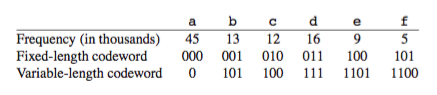
\includegraphics[width = 16.5cm, height = 6cm]{1.png}
\centering \linebreak \linebreak {\small Figure 1.1.0: {\bfseries (a)} A graph representing the vertices, edges, and faces of a dodecahedron, with a {\bfseries Hamiltonian Cycle} shown by shaded edges. {\bfseries (b)} A bipartite graph with an odd number of vertices. Any such graph is non-hamiltonian.} \hfill \break
\end{figure} \hfill \break

The dodecahedron is {\bfseries Hamiltonian}, and Figure 1.1.0 {\bfseries (a)} shows one {\bfseries Hamiltonian Cycle}. Not all graphs are {\bfseries Hamiltonian}, however. For example, Figure 1.1.0 {\bfseries (b)} shows a bipartite graph with an odd number of vertices. \hfill \break 

We can define the {\bfseries hamiltonian-cycle problem}, “Does a graph G have a Hamiltonian cycle?” as a formal language: \hfill \break

\begin{center}
HAM-CYCLE = $\lbrace$ ( G ) : G is a {\bfseries Hamiltonian} Graph $\rbrace$
\end{center} \hfill \break

How might an algorithm decide the language HAM-CYCLE? Given a problem instance $\langle\ G\ \rangle$, one possible decision algorithm lists all permutations of the vertices of {\itshape G} and then checks each permutation to see if it is a Hamiltonian path. What is the running time of this algorithm? If we use the “reasonable” encoding of a graph as its adjacency matrix, the number {\bfseries m} of vertices in the graph is $\Omega ( \sqrt{n} )$, where $n\ =\ \vert \langle G \rangle \vert$ is the length of the encoding of {\itshape G} There are {\bfseries m!} possible permutations of the vertices, and therefore the running time is $\Omega ( m! )$ = $\Omega ( \sqrt{n} )$  = $\Omega ( 2^{\sqrt{n}} )$, which is not {\bfseries $\mathcal{O}(n^{k})$} for any constant {\itshape k}. Thus, this naive algorithm does not run in polynomial time. In fact, the {\bfseries hamiltonian-cycle problem} is NP-complete.

\subsection{Verification Algorithms:}

Consider a slightly easier problem. Suppose that a friend tells you that a given graph {\itshape G} is {\bfseries Hamiltonian}, and then offers to prove it by giving you the vertices in order along the hamiltonian cycle. It would certainly be easy enough to verify the proof: simply verify that the provided cycle is hamiltonian by checking whether it is a permutation of the vertices of V and whether each of the consecutive edges along the cycle actually exists in the graph. You could certainly implement this verification algorithm to run in {\bfseries $\mathcal{O}(n^{2})$} time, where {\itshape n} is the length of the encoding of {\itshape G}. Thus, a proof that a {\bfseries Hamiltonian Cycle} exists in a graph can be verified in polynomial time. \hfill \break

We define a {\bfseries verification algorithm} as being a two-argument algorithm {\itshape A}, where one argument is an ordinary input string {\itshape x} and the other is a binary string {\itshape y} called a certificate. A two-argument algorithm {\itshape A} verifies an input string {\itshape x} if there exists a certificate {\itshape y} such that {\bfseries A ( x, y ) = 1}. The {\bfseries language verified} by a verification algorithm A is: \hfill \break

\begin{center}
L = $\lbrace$ {\itshape x} $\in$ $\lbrace$ 0, 1 $\rbrace ^{*}$ : there exists {\itshape y} $\in$ $\lbrace$ 0, 1 $\rbrace ^{*}$ such that {\itshape A ( x, y ) = 1} $\rbrace$
\end{center} \hfill \break

Intuitively, an algorithm {\itshape A} verifies a language {\bfseries L} if for any string {\itshape x} $\in$ {\itshape L}, there exists a certificate {\itshape y} that {\itshape A} can use to prove that {\itshape x} $\in$ {\itshape L}. Moreover, for any string {\itshape x} $\not \in$ {\itshape L}, there must be no certificate proving that {\itshape x} $\in$ {\itshape L} . For example, in the {\bfseries Hamiltonian-Cycle problem}, the certificate is the list of vertices in some Hamiltonian Cycle. If a graph is Hamiltonian, the Hamiltonian Cycle itself offers enough information to verify this fact. Conversely, if a graph is not-hamiltonian, there can be no list of vertices that fools the verification algorithm into believing that the graph is Hamiltonian, since the verification algorithm carefully checks the proposed “cycle” to be sure.

\pagebreak